To design a database schema we must first understand it, for understanding we design ER programs, they stand for Entity Relationship Diagrams.
An ER diagram would be absolutely helpful in defining relationships so that we can understand the relations, object and attributes associated with each table in our database.
ER diagrams act as a middle man between the requirements and the actual schema that gets implemented.
\begin{itemize}
    \item ER diagrams consists of different shapes and symbols that establish relationships.
    \item An entity is an object we want to model and store information about. In ER diagrams they are modeled using a square or rectangle.
\end{itemize}

\begin{itemize}
    \item ER Diagrams: used to design the database, it is used to model an entity.
    \item An entity is depicted as a square, in this example the entities we want to model are students.
        \begin{figure}[H]
            \centering
            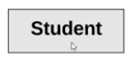
\includegraphics[width=0.4\textwidth]{./Figs/2020-12-23-23-33-10.png}
        % 	\caption{}
        \end{figure}
        
    \item An attribute is a specific piece of information about an entity. In ER diagrams they are modeled using ovals connected to entity.
        \begin{figure}[H]
            \centering
            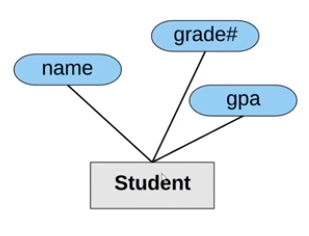
\includegraphics[width=0.4\textwidth]{./Figs/2020-12-23-23-33-26.png}
        % 	\caption{}
        \end{figure}
    \item Primary key: an attribute that uniquely identifies an entry in the database table. Modeled inside an oval, the primary key name is underlined.
        \begin{figure}[H]
            \centering
            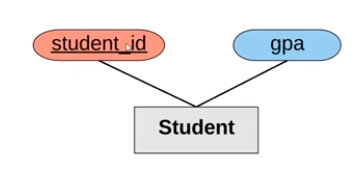
\includegraphics[width=0.4\textwidth]{./Figs/2020-12-23-23-33-54.png}
        % 	\caption{}
        \end{figure}
    \item Composite attributes: Attributes that can be broken up into sub-attributes. In this example the name attribute can be broken up further into first name and last name, this is a composite attribute.
        \begin{figure}[H]
            \centering
            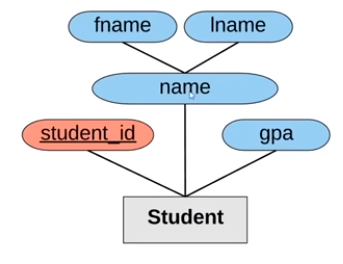
\includegraphics[width=0.4\textwidth]{./Figs/2020-12-23-23-34-47.png}
        % 	\caption{}
        \end{figure}
    \item Multi-valued attribute: an attribute that can have more than one value. Modeled with an oval with an inner oval. In this case ``clubs'' is a multi-values attribute because a student could be involved in more than one club or zero, it can have more than one value, they are not going to have more than one gpa or more than one name, but they can be involved in more than one club.
        \begin{figure}[H]
            \centering
            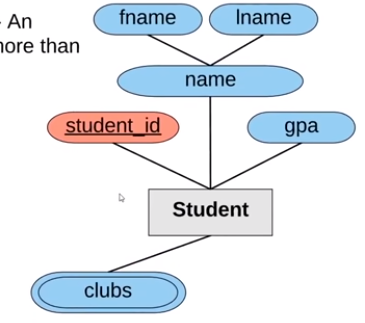
\includegraphics[width=0.4\textwidth]{./Figs/2020-12-23-23-35-38.png}
        % 	\caption{}
        \end{figure}
    \item Derived attribute: an attribute that can be derived from the other attributes, modeled using oval with dashed lines. A derived attribute is not stored in the database, they can be figured out whenever they are needed but for the sake of efficient memory usage they are not stored because they can be derived whenever they are needed. Has honors can be derived from the gpa.
        \begin{figure}[H]
            \centering
            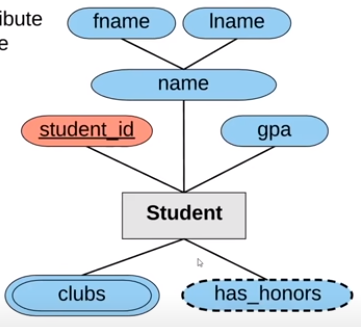
\includegraphics[width=0.4\textwidth]{./Figs/2020-12-23-23-37-32.png}
        % 	\caption{}
        \end{figure}
    \item Multiple entities: you can define more than one entity in the diagram. We can have multiple entities and establish relations between them, in this case lets define an entity called class. Notice the class entity has a primary key called class id.
        \begin{figure}[H]
            \centering
            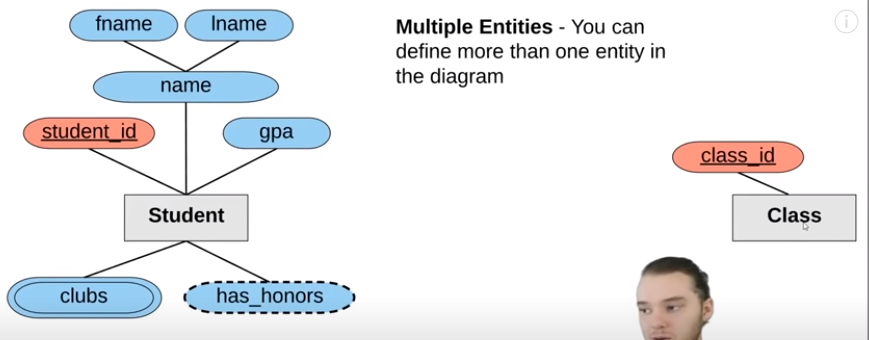
\includegraphics[width=0.4\textwidth]{./Figs/2020-12-23-23-40-02.png}
        % 	\caption{}
        \end{figure}
    \item Relationship: defines a relationship between two entities. Modeled using lines and a diamond shape. Using a double line means that task has total and one line means partial. When we have two or more entities we can define relationships between those two entities, here lets establish a relationship between student and class:
        \begin{itemize}
            \item A relationship is denoted by the diamond, in this case ``takes'', the lines connecting the entities to the relationship also hold particular information. 
            \item The relationship here is that a student can take a class and a class can be taken by a student.
            \item In many ways relationships are denoted as verbs, and they can go both ways, in this case you can say the student takes a class and the class takes a student.
            \item One line means partial participation, meaning that not all students need to take a class.
            \item Two lines means total participation, meaning that all the classes need to be taken by at least a minimum of students, it doesn't make sense to have a class that has zero students taking it.
        \end{itemize}
        \begin{figure}[H]
            \centering
            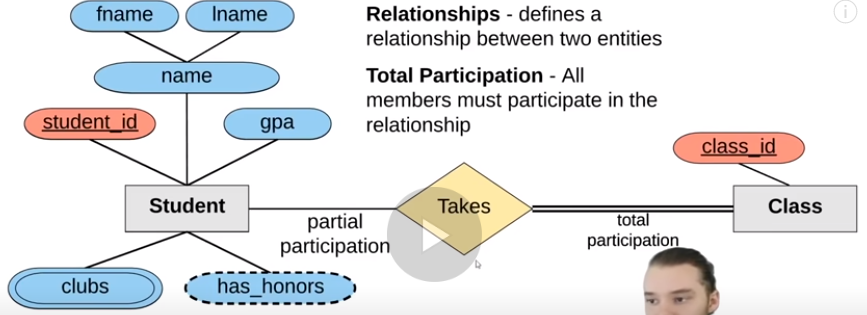
\includegraphics[width=0.4\textwidth]{./Figs/2020-12-23-23-41-52.png}
        % 	\caption{}
        \end{figure}
    \item Relationship attribute: an attribute about the relationship. In this case there is an attribute on the relationship, the entity student takes a class, while he takes the class the entity student will receive a grade, this only happens when the student takes the class. It doesn't make sense to store in student grades on classes he never took or never will.
        \begin{figure}[H]
            \centering
            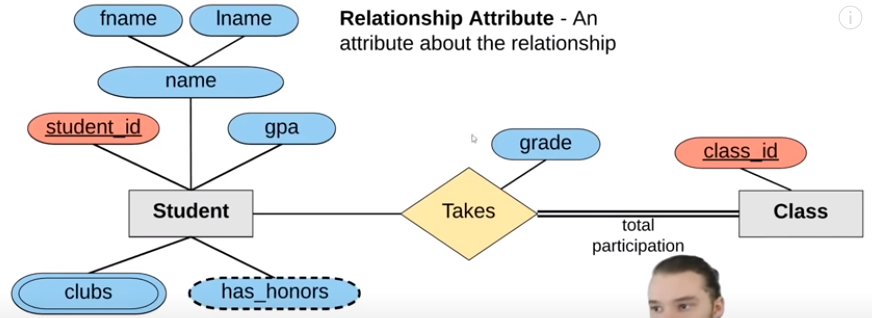
\includegraphics[width=0.4\textwidth]{./Figs/2020-12-23-23-47-13.png}
        % 	\caption{}
        \end{figure}
    \item Relationship cardinality: the number of instances of an entity from a relation that can associated with the relation. This means for our example that a student can take multiple classes, and we can define the same thing for the class, we can say the class is taken by any number of students. However, we can define cardinality relationships as the following:
        \begin{itemize}
            \item 1:1, meaning that a student can take one class and a class can be taken one student. This means that the class can only have one student and the student can only take one class. Doesn't make very much sense in this example.
            \item 1:N, N meaning a constant number of students, 1:N means that a student can take one class and a class can be taken by N number of students.
            \item N:M, means that a student can take any number of classes and a class can be taken by any number of students.
            \item This is relevant because it is useful in data modeling requirements, for example if you require your database to check that a student can only take one class at a time, then that is something you want to consider in your ER diagrams.
        \end{itemize}
        \begin{figure}[H]
            \centering
            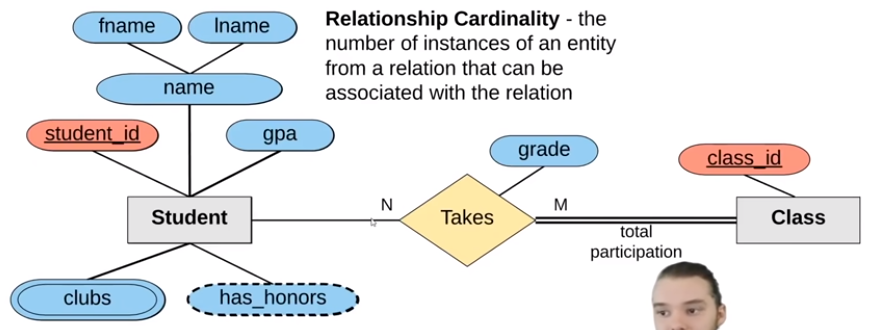
\includegraphics[width=0.4\textwidth]{./Figs/2020-12-23-23-52-17.png}
        % 	\caption{}
        \end{figure}
    \item Weak entity: an entity that cannot be uniquely identified by its attributes alone, an entity that will depend on another.
        \begin{itemize}
            \item In this example a weak entity is an exam, notice that a class can have an exam, the exam is an entity, the exam has the primary key of exam id, but in this case an exam can't exist without a class, in order for an exam to exist it has to be associated with a class.
        \end{itemize}
        \begin{figure}[H]
            \centering
            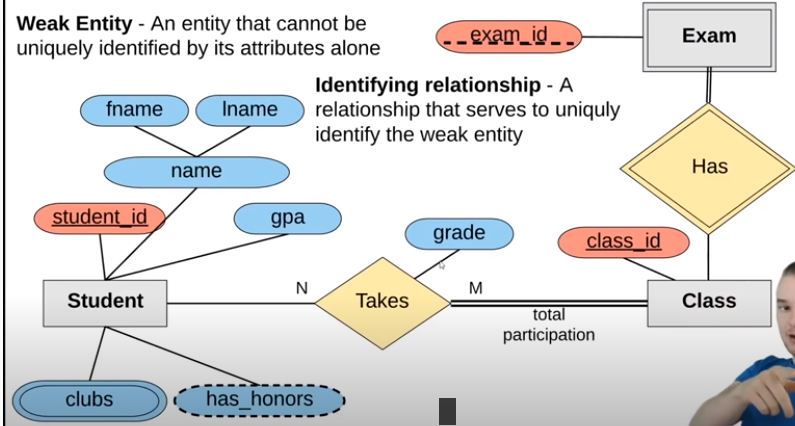
\includegraphics[width=0.4\textwidth]{./Figs/2020-12-23-23-53-53.png}
        % 	\caption{}
        \end{figure}
    \item Identifying relationship: a relationship that serves to uniquely identify the weak entity.
        \begin{itemize}
            \item In this example the identifying relationship is the ``has'', an exam can be uniquely \emph{identified} only if there is a class associated with it. 
            \item The exam does not exist on its own, it relies on a class for an identity.
            \item Whenever we have a weak entity and identifying relationship the weak entity always has to have total participation in the identifying relationship, all exams must have a class but not all classes need to have an exam.
        \end{itemize}
        \begin{figure}[H]
            \centering
            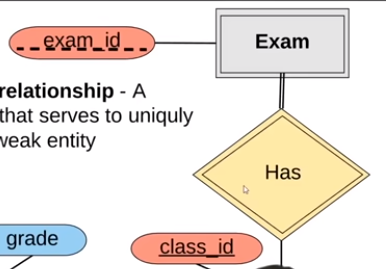
\includegraphics[width=0.4\textwidth]{./Figs/2020-12-23-23-55-58.png}
        % 	\caption{}
        \end{figure}
\end{itemize}

Knowing this, we can take this ER diagram and convert it to a actual database schema.
